% -*- TeX-PDF-mode: t; TeX-engine: xetex; IspellDict: english -*-
% Bypasses bug in geometry package?
\makeatletter\let\ifGm@compatii\relax\makeatother
\documentclass[10pt, compress]{beamer}

\usetheme[usetitleprogressbar]{metropolis}


\usepackage[english]{babel}

\usepackage{array}
\usepackage{graphicx}
\usepackage{dsfont}
\usepackage{mathbbol}
\usepackage{amsfonts}
\usepackage{color}
\usepackage{verbatim}
\usepackage{cite}
\usepackage{appendixnumberbeamer}
\usepackage{xspace}
\usepackage{tikz}
\usepackage{listingsutf8}
\lstset{escapeinside={(*@}{@*)}}
\usepackage{longtable}
\usepackage{framed}
\definecolor{shadecolor}{rgb}{0.9,0.9,0.9}

\definecolor{emphcolor}{rgb}{0.65,0.78,0.29}

\newcommand\blfootnote[1]{%
  \begingroup
  \renewcommand\thefootnote{}\footnote{#1}%
  \addtocounter{footnote}{-1}%
  \endgroup
}

\usepackage{booktabs}
\usepackage[scale=2]{ccicons}

\usepackage{pgfplots}
\usepgfplotslibrary{dateplot} 

\metroset{block=fill}

\usepackage{xspace}
\newcommand{\themename}{\textbf{\textsc{metropolis}}\xspace}

\setbeamertemplate{section in toc}{%
    ∙  \inserttocsection \par}

\usepgfplotslibrary{dateplot}

\title[Guiding patrol drones]{Detecting fire with drones}
\author{\textbf{E}ma, \textbf{N}ikola, \textbf{I}sabel and \textbf{A}lba
  \textbf{C}oding (ENIAC)}
\date{\textbf{womENcourage 2018, Belgrade}}


\renewcommand<>{\emph}[1]{{\textbf{\color{orange}{\only#2#1}}}‌​}
%\renewcommand<>{\emph}[1]{{\color{emphcolor}{\only#2{\itshape}#1}}‌​}

\begin{document}

\maketitle

\listoftables

% Intro %%%%%%%%%%%%%%%%%%%%%%%%%%%%%%%%%%%%%%%%%%%%%%%%%%

\begin{frame}{Goal}

 
  Prevent fires by:
  \vspace{-2mm}
  \begin{itemize}
  \item Providing \textbf{tools to help forest guards}.
  \item Using drones to \textbf{automatically patrol vulnerable areas}.
  \end{itemize}
  
  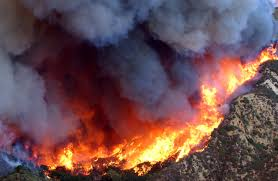
\includegraphics[width=0.6\textwidth]{california_fire.jpg}
%
  \blfootnote{https://upload.wikimedia.org/wikipedia/commons/9/98/Simi\_Valley\_fire\_California\_USA.jpg}
\end{frame}


\begin{frame}{Step 1 -- Build a model}

  \begin{itemize}
    \item Find a dataset. \textbf{Montesihno Park} contains:
      \begin{itemize}
      \item Historic information of fire and weather characteristics.
      \item Data distributed in a grid.
      \end{itemize}

      \begin{figure}
        \centering 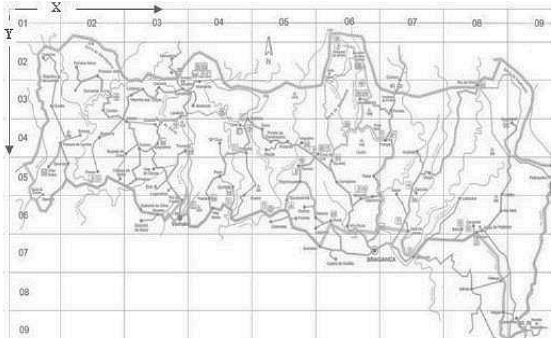
\includegraphics[width=0.5\textwidth]{park}
      \end{figure}
    \item Use supervised machine learning (linear regression) to infer a
      function for the \textbf{probability of fire}.
\end{itemize}
\end{frame}


\begin{frame}{Step 2 -- Help forest guards}

  Use the \textbf{model} and the information from the \textbf{sensors} in the park to \textbf{build a risk map} with probability of fire.

  \begin{figure}[h]
    \vspace{-3mm}
    \centering
    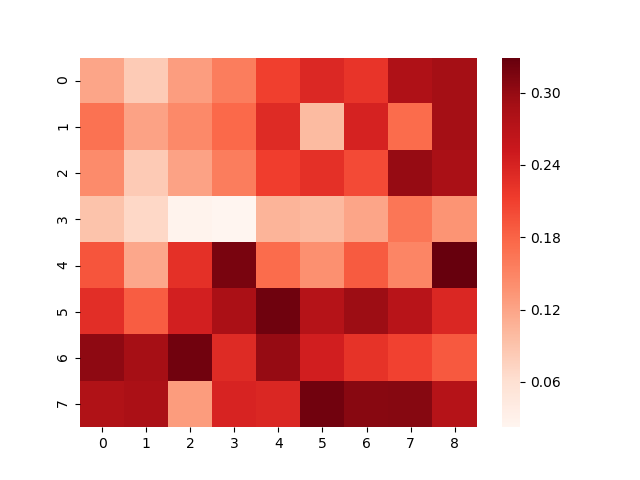
\includegraphics[width=0.6\textwidth]{../images/Figure_summer}
    \vspace{-5mm}
  \end{figure}
  To be used by forest guards to: 
  \begin{itemize}
  \item \textbf{distribute available resources},
  \item \textbf{clean the area} (e.g., remove dry plants),
    \item ...
  \end{itemize}
\end{frame}

\begin{frame}{Step 3 -- Patrol Automatically}

  The \textbf{drone} uses the probability of fire to \textbf{patrol
    automatically the most vulnerable areas}.

  \medskip
  \begin{Large}
    \textbf{DEMO}
  \end{Large}
  
  \pause
  \medskip
  \textbf{Future work}:
  \begin{itemize}
  \item \textbf{take pictures}, to be checked by the forest guards.
  \item \textbf{recognize fire} in the pictures using image recognition algorithms.
  \end{itemize}
\end{frame}

\begin{frame}{Summary -- What did we do?}

\large
  \begin{itemize}
  \item \textbf{Found a dataset} of fires in Mountesihno Park.
  \item \textbf{Processed} the data.
  \item \textbf{Built a model} of the \textbf{risk of fire}.
  \item Built a \textbf{visualization tool} for the forest guards.
  \item Programmed a \textbf{patrolling algorithm} (using ROS).
  \end{itemize}

  \centering

  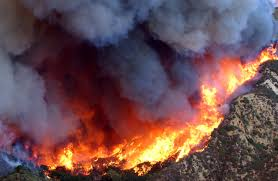
\includegraphics[width=0.2\textwidth]{california_fire.jpg}
  \hspace{2mm}
  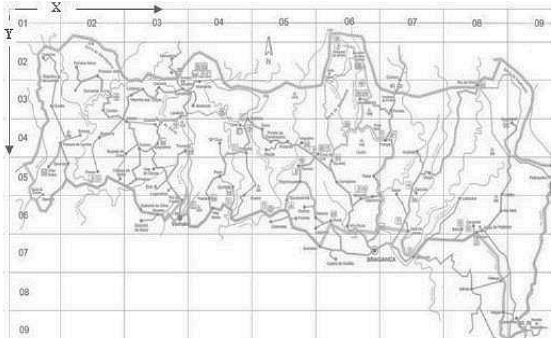
\includegraphics[width=0.2\textwidth]{park}
    \hspace{2mm}
    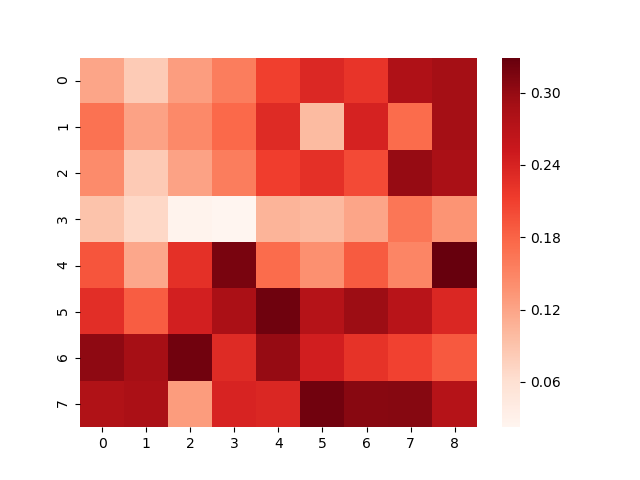
\includegraphics[width=0.2\textwidth]{../images/Figure_summer}
    \hspace{2mm}
  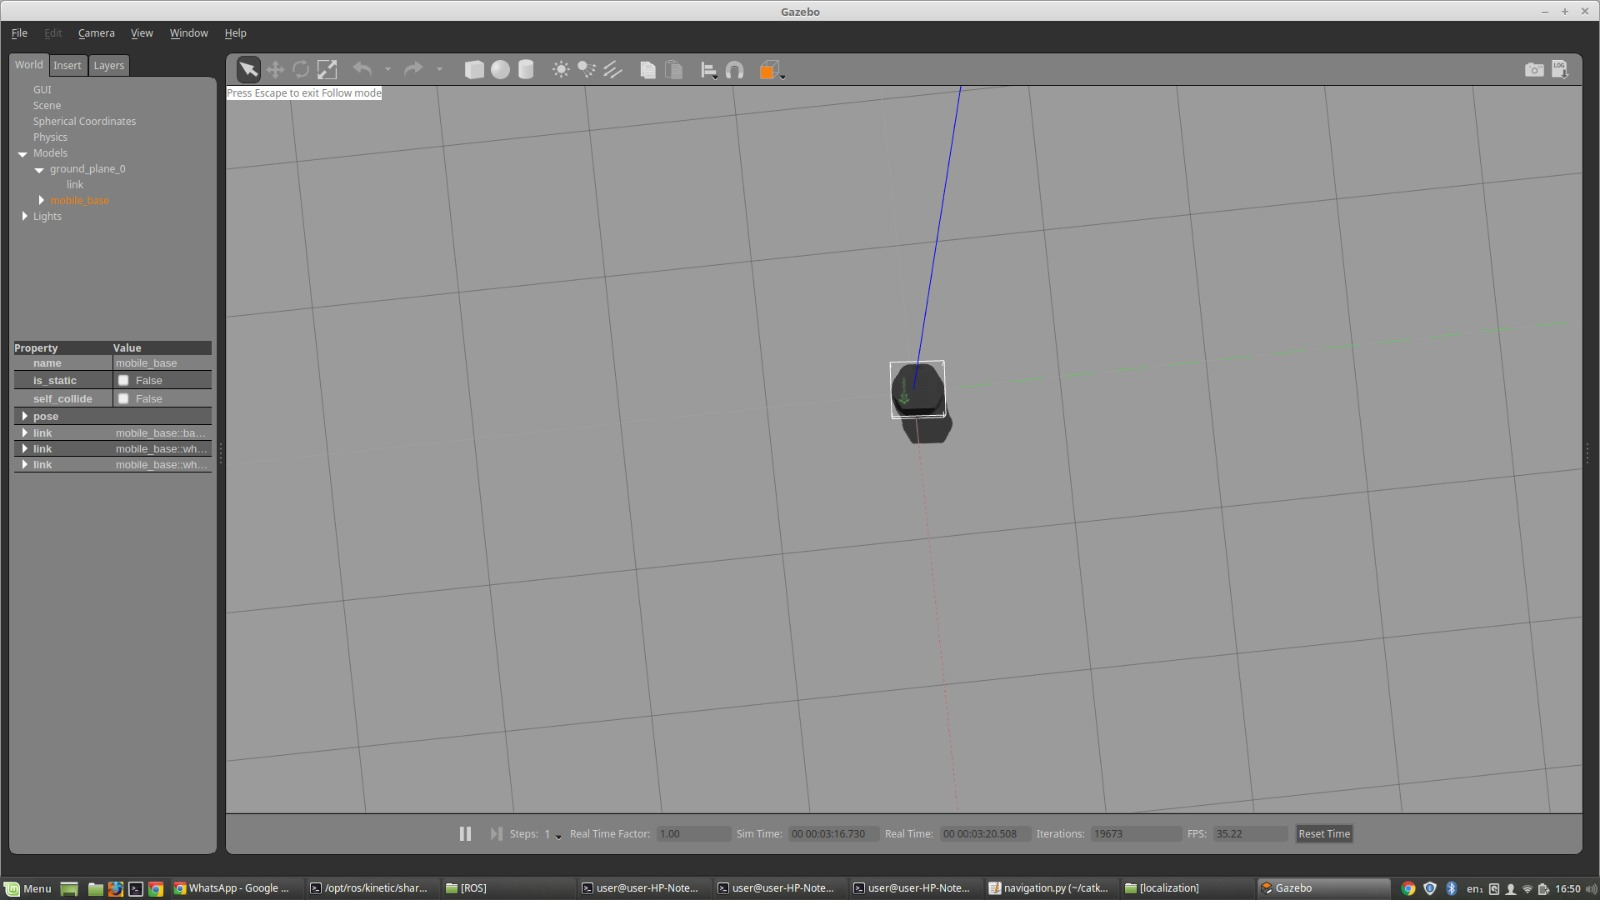
\includegraphics[width=0.2\textwidth]{robot}
  
\end{frame}

\end{document}

%%% Local Variables:
%%% mode: latex
%%% TeX-master: t
%%% End:

